\documentclass[conference]{IEEEtran}
\IEEEoverridecommandlockouts
% The preceding line is only needed to identify funding in the first footnote. If that is unneeded, please comment it out.
\usepackage{cite}
\usepackage{amsmath,amssymb,amsfonts}
\usepackage{algorithmic}
\usepackage{graphicx}
\usepackage{textcomp}
\usepackage{xcolor}
\def\BibTeX{{\rm B\kern-.05em{\sc i\kern-.025em b}\kern-.08em
    T\kern-.1667em\lower.7ex\hbox{E}\kern-.125emX}}
\begin{document}

\title{Quantum Binary Networks Evaluation\\ with Deutsch - Jozsa's Algorithm\\
{\footnotesize \textsuperscript{*}Note: Sub-titles are not captured in Xplore and
should not be used}
\thanks{Identify applicable funding agency here.
If none, delete this.}
}

\author{\IEEEauthorblockN{1\textsuperscript{st} Given Name Surname}
\IEEEauthorblockA{\textit{dept. name of organization (of Aff.)} \\
\textit{name of organization (of Aff.)}\\
City, Country \\
email address or ORCID}
\and
\IEEEauthorblockN{2\textsuperscript{nd} Given Name Surname}
\IEEEauthorblockA{\textit{dept.
name of organization (of Aff.)} \\
\textit{name of organization (of Aff.)}\\
City, Country \\
email address or ORCID}
\and
\IEEEauthorblockN{3\textsuperscript{rd} Given Name Surname}
\IEEEauthorblockA{\textit{dept.
name of organization (of Aff.)} \\
\textit{name of organization (of Aff.)}\\
City, Country \\
email address or ORCID}
\and
\IEEEauthorblockN{4\textsuperscript{th} Given Name Surname}
\IEEEauthorblockA{\textit{dept.
name of organization (of Aff.)} \\
\textit{name of organization (of Aff.)}\\
City, Country \\
email address or ORCID}
\and
\IEEEauthorblockN{5\textsuperscript{th} Given Name Surname}
\IEEEauthorblockA{\textit{dept.
name of organization (of Aff.)} \\
\textit{name of organization (of Aff.)}\\
City, Country \\
email address or ORCID}
\and
\IEEEauthorblockN{6\textsuperscript{th} Given Name Surname}
\IEEEauthorblockA{\textit{dept.
name of organization (of Aff.)} \\
\textit{name of organization (of Aff.)}\\
City, Country \\
email address or ORCID}
}

\maketitle

\begin{abstract}
The Deutsch-Jozsa's quantum algorithm allows determining if a function is constant or balanced with a single function call.
In this paper, we show how to apply Deutsch-Jozsa's algorithm to evaluate Quantum Binary Neural Networks (QBNN).
We define a probabilistic algorithm for a QBNN evaluation that receives test patterns in a quantum superposition.
It plucks probabilistic information with a constant number of executions.
The goal is to present possible new directions on quantum machine learning research.
\end{abstract}

\begin{IEEEkeywords}
quantum computation, quantum binary neural networks, evaluation,
\end{IEEEkeywords}

\section{Introduction}\label{sec:introduction}
Evaluating the outcomes of a classification algorithm is one of the most important steps to validate its
efficiency~\cite{japkowicz2006question}.
Time is an important factor, mainly in
real-time applications that are updated constantly by new data and must have a fast evaluation~\cite{chen2012classifier}.
To handle this issue, quantum algorithms have shown be able to solve some problems more efficiently than classical algorithms
~\cite{deutsch1992rapid}.

In some cases, quantum algorithms can solve some problems more efficiently than classical algorithms
~\cite{deutsch1992rapid}.
One proof of the quantum speedup is the Deutsch-Jozsa's algorithm.
It is a method to determine whether a binary function is constant or balanced.
While classical computer solves with complexity \(\mathcal{O}(2^{n})\),
the Deutsch - Jozsa's algorithm does it with \(\mathcal{O}(1)\) iterations.

This research aims to evaluate the possibility to use data in superposition to evaluate a classifier.
We use a Quantum Binary Neural Network (QBNN)~\cite{fawaz2019training}, by checking whether all the inputs are correctly
classified by using Deutch-Josza's approach.
We adopt the hypothesis of once having a QBNN we use it as the oracle of the Deutch - Josza's algorithm.
The following sections are

Section~\ref{sec:qc}: gives an introduction to quantum computation
Section~\ref{sec:deutsch-jozsa's-algorithm}: gives an introduction of the Deutsch-Jozsa's algorithm
Section~\ref{subsec:quantum-neuron-evaluation}: presents a quantum binary neuron and its evaluation
Section~\ref{sec:quantum-binary-neural-networks-evaluation}: shows the implementation of a QBNN evaluation
Section~\ref{sec:conclusion}: presents a final analysis of the results and further directions.

\section{Quantum computing}\label{sec:qc}
%qubits, operators, measure, deutch-josza
\subsection{What's quantum computation?}\label{subsec:what's-quantum-computation?}

Classical computation relies on the use of the smallest unit of information known as the bit, which can assume values of
0 or 1.
While that, in the quantum computation we have quantum bits known as qubits, those can
assume the values of 0 and 1 simultaneously.
That and other quantum properties give us the abilities that cannot be achieved in the classical computation.
Also, these new tools make us able to deal better with problems of the classical world that are difficult
to solve with today's classical algorithms~\cite{russon_2017,deutsch1992rapid}.

\subsection{Fundamentals}\label{subsec:fundamentals}

\subsection{Qubits and Superposition}\label{subsec:qubits-and-superposition}

\textit{Definition:} Qubits have are different from the bits and thus are represented in a specific form.
They are represented as \(a|\uparrow\rangle + b|\rightarrow\rangle\), where \(a\) and \(b\) are complex
numbers and \(|\uparrow\rangle\) and \(|\rightarrow\rangle\) are vectors that represents the values:

\[ |0\rangle = \begin{bmatrix} 1 \\ 0\end{bmatrix}  |1\rangle = \begin{bmatrix} 0 \\ 1\end{bmatrix}\]

Therefore, we have a probability of \(|a|^2\) to our vector be found at state \(|0\rangle \) and
\(|b|^2\) in the state \(|1\rangle\).
When both vectors are not null we say that the qubit is in \textit{superposition}, it means that both states
\(|0\rangle\) and \(|1\rangle\) are represented simultaneously.
It can be done with only one qubit or several n qubits at once what is called
\textit{superposition of n qubits}~\cite{yanofsky2008quantum,rieffel2014quantum}.
When we try to handle with a qubit in superposition or not to determine its state we make the
qubit collapse to one of the state \(|0\rangle\) or \(|1\rangle\) and we call that
\textit{measurement}~\cite{yanofsky2008quantum,rieffel2014quantum}.

\subsection{Quantum Gates}\label{subsec:quantum-gates}

\textit{Definition:} A \textit{quantum gate} is simply an operator that acts on a single qubit and they are
represented for unitary matrix.
Unitary matrix is a matrix that \(U\star U^\dagger = I\) where
\(U^\dagger\) is the combination of transpose and conjugate operation of the matrix \textit{U}.
Some operation can be done only with a qubit like the  Not (X) and Hadamard (H)~\cite{yanofsky2008quantum},
those are known as \textit{single qubit operations}.
Some other kinds of operation require two or more qubits to be done as the \textit{controlled operation}.


An example of a single-qubit operation is the X gate that turns the qubit from \(|0\rangle\) to
\(|1\rangle\) and vice-versa.
Another example of the same kind of operation is the H gate, that can turn a qubit into \textit{superposition} of
different states.
It transforms the state \(|0\rangle\) in \(\frac{|0\rangle + |1\rangle}{\sqrt{2}}\) and the state
\(|1\rangle\) in \(\frac{|0\rangle - |1\rangle}{\sqrt{2}}\).
It also important to note that a Hadamard operation can be applied to more than one states at once and the operation is
represented for \(H^{\oplus n}\).
By the other hand, an example of controlled operation we have the \textit{CNot} that having the state \(|xy\rangle\) the second state
\(|y\rangle\) (target) is changed if the first qubit \(|x\rangle\) (control) is one~\cite{yanofsky2008quantum}.


\section{Deutsch-Jozsa's Algorithm}\label{sec:deutsch-jozsa's-algorithm}

\subsection{The problem}\label{subsec:the-problem}

The problem that the  Deutsch-Jozsa's algorithm tries to solve is given a binary function
\(f:\{{0,1\}}^n \rightarrow \{0,1\}\), determine if the function is constant or not.
We also consider that the output is always 0 or 1 and \textit{n} is the number of possible inputs to such function.
We determine if it is constant (all inputs are always only 0 or 1) or balanced
(half inputs are 0 and the other half 1) as the rule of the function is unknown~\cite{benatti2003deciding,deutsch1992rapid}.


\subsection{Finding a Solution}\label{subsec:finding-a-solution}

 Assuming that we have a binary function \(f: \{{0,1\}}^n \rightarrow  \{0,1\}\).
 A classical solution for this problem would required us to evaluate in the worse case \(2^{n-1} + 1\)
 inputs, thus requiring \(\mathcal{O}(2^{n})\) classical evaluations~\cite{yanofsky2008quantum,deutsch1992rapid}.
  % N + 1 with N invocations of the function \cite{deutsch1992rapid}

 Even though a classical solution to this problem is costly, the quantum computation can give us a new form to deal with
the problem.
A quantum solution is based on the quantum parallelism where we can evaluate different outputs in just one evaluation of
the function~\cite{deutsch1992rapid}.
 First of all we consider that \(\{{|a,b\rangle\}}(a \in \{{0,1\}}^n, b \in \{0,1\})\) is a orthonormal
 basis in the Hilbert space~\cite{deutsch1992rapid}.
 The function \(U_f\) can effect the states of the
 basis that we are using such that \(|a,b\rangle \rightarrow |a,b \oplus f(a) \rangle\),
 where \(\oplus\) is a bit-wise operation~\cite{deutsch1992rapid}.


 It is also considered \textit{n} as a natural number and \(U_f\) a function defined as
 \(f:\{{0,1\}}^n \rightarrow \{{0,1\}}\), where \(\{{0,1\}}^n\) is every combination of \(n\) qubits.

 Based on the~\cite{deutsch1992rapid} proposal we can affirm certainly that after measuring the qubits
 what will be found is that one of the following statements is true.

 1. \(U_f\) is not constant at 0 or 1.

 2. \(U_f\) gives not zero as response for the in the sequence f(00\dots0), f(00\dots1), \dots, f(0\dots11).

 To obtain one of the above results, we follow the hypothesis of having \(|\psi\rangle\) state defined as a
 superposition of many states as follows:

 \begin{equation}
    |\psi\rangle = \sum_{j=0}^{2n-1} \frac{|\textbf{x},0\rangle}{\sqrt{2^n}}
 \end{equation}
 where \textbf{x} is every combination of \textit{n} bits~\cite{deutsch1992rapid}.

 After that, we apply \(U_f\) which is defined as:

 \begin{equation}
    U_f = \sum_{j=0}^{2n-1} \frac{{(-1)}^{f(\textbf{x})}|\textbf{x},0\rangle}{\sqrt{2n}}
 \end{equation}

 The operation above changes the phase of the states and it makes possible for us to verify if a function is constant or
 not.
 The function is constant if the magnitude of the inner product is equal to
 \(\pm 1\)~\cite{deutsch1992rapid,yanofsky2008quantum}.
 The function is balanced if the magnitude of the inner product between the initial state \(|\psi\rangle\)
 and \(U_f\) is exactly half part of the states have phase on 1 and the other half on -1.

 It will make one-half cancel with another half of qubits and produce some output different from zero after the
 measurement~\cite{deutsch1992rapid,nielsen2002quantum}.

 That is also possible to estimate the final state of the n-qubit of input by the following equation:

\renewcommand{\figurename}{Fig.}
 \begin{figure}[ht!]
     \begin{equation}
        |\psi\rangle = \sum_{z=0}^{2^{n-1}} \Bigg(\sum_{x=0}^{2^{n-1}} \frac{{(-1)}^{x.z +f(x)}}{2^n}\Bigg)|z\rangle
    \end{equation}
     \caption{Considering \(x.z\) as a bit-wise inner product and \(\{|z\rangle\}\) a computational basis
     ~\cite{benatti2003deciding}.
     The probability of obtaining \(z=0\) indicates the probability of our function be constant.}
 \end{figure}

\subsection{Initial Considerations}\label{subsec:quantum-neuron-evaluation}

 First, we consider some modification of the ~\cite{fawaz2019training} approach.
Differently of the quantum neuron proposed by~\cite{fawaz2019training} we load all inputs and the accuracy qubit in
superposition as in the~\cite{Trugenberger_2001} approach, while that, the weights are loaded one by one.
It will allow us to evaluate all the answers for each combination of binary weights separately.
The second important modification is that instead of use the weights as control and inputs as target in the multiplication
between weights and inputs we use the inputs as control and weights as target.

\section{Quantum Neuron Evaluation}\label{sec:quantum-neuron-evaluation}

 We made a small scale test using a quantum neuron based on~\cite{fawaz2019training} approach and further we evaluated
 the whole QBNN\@.
 At this stage we are evaluation a quantum neuron with two inputs and weights and its activation function.
 We loaded the expected result set it first to one and wherever it should be one we set to zero~\cite{fawaz2019training}.
 This way we will have 1 whatever the neuron yields the correct output and 0 where not just as in the paper we mentioned.

 \subsection*{Toy Problem}
    We considered a toy problem based on~\cite{fawaz2019training}, where \(sign(x_1 + x_2)\) and the function returns one
    if \(sign(x_1 + x_2) \geq 0\) and 0, otherwise.\footnote{The values are binary 1 and -1 that are represented as 1
    and 0 respectively.}

\subsection{Initial Setup}\label{subsec:initial-setup}


The initial state consists of \(|\psi_0\rangle = |11\rangle|00\rangle|1\rangle\Big[\frac{|0\rangle - |1\rangle}{\sqrt{2}}\Big]\).
We are considering in this case the state \(|11\rangle\) as the weights, \(|00\rangle\) the inputs, the expected outcome \(|1\rangle\), and
\(\Big[\frac{|0\rangle - |1\rangle}{\sqrt{2}}\Big]\) the ancillary qubit.
Now we can apply the Hadamard operation in the inputs states and a not gate in the weights to load the inputs and the weights.

\begin{equation}
|\psi_1\rangle = \frac{1}{2}(|00\rangle|000\rangle + |00\rangle|010\rangle + |00\rangle|100\rangle + |00\rangle|110\rangle)
|a\rangle
\end{equation}

After, we load the accuracy for each input setting to zero the state where must outcome \(|1\rangle\) and one where the
expected output is the state $|0\rangle$~\cite{fawaz2019training}.
It can be achieved using a Toffoli and two not gates.\footnote{Toffoli gates is similar to c-not, but used when we have
two control qubits and one target~\cite{yanofsky2008quantum}.}
This form when we apply the weights and the activation function we will obtain the accuracy entangled with which input
making a possible an evaluation based on the original paper proposal.
Then \(|\psi_2\rangle\) is given by:

\begin{equation}
|\psi_2\rangle = \frac{1}{2}(|00\rangle|001\rangle + |00\rangle|010\rangle + |00\rangle|100\rangle + |00\rangle|110\rangle)
|a\rangle
\end{equation}

\subsection{Oracle Application}\label{subsec:oracle-application}

The oracle that we are considering in this step is our neuron implementation of two inputs and two weights.
Thus we then apply the weights to every input which are in superposition.
Differently of~\cite{fawaz2019training} proposal we choose a single set of two qubits to be applied in this example its 11.
The result obtained is the state $|\psi_3\rangle$ shown below

% modificar explicação
\begin{equation}
|\psi_3\rangle = \frac{1}{2}(|00\rangle|001\rangle + |01\rangle|010\rangle + |10\rangle|100\rangle + |11\rangle|110\rangle)
|a\rangle
\end{equation}

At this stage, we must apply the majority function as proposed for~\cite{fawaz2019training} and obtain the accuracy of
the QBNN

\begin{equation}
|\psi_3\rangle = \frac{1}{2}(|00\rangle|001\rangle + |01\rangle|011\rangle + |10\rangle|101\rangle + |11\rangle|111\rangle)
|a\rangle
\end{equation}

It is clear at this point that the QBNN algorithm produced a balanced output marking correctly half part of the answers.
Then we evaluate the algorithm output by the application of a c-not gate into the ancillary qubit.
It will change the signal of the states with the correct output such that \((-1)^{f(x)}|x\rangle\).

\begin{equation}
|\psi_3\rangle = \frac{1}{2}(-|00\rangle|001\rangle - |01\rangle|010\rangle - |10\rangle|100\rangle - |11\rangle|110\rangle)
|a\rangle
\end{equation}

Now considering the reverse order we will apply all the operation before the last c-not gate and obtain the following state.

\begin{equation}
|\psi_3\rangle = |11\rangle\frac{1}{2}(-|001\rangle - |010\rangle - |100\rangle - |110\rangle)
|a\rangle
\end{equation}

\subsection{Retrieving Information}\label{subsec:neuron-evaluation}

Now as part of the evaluation we apply the Hadamard transform again in the input states, just as in equation (3).
Given the inputs and accuracy \(-|001\rangle, -|011\rangle, - |101\rangle, -|111\rangle\), after the Hadamard, we will have
all \(|00\rangle\) states with magnitude -1.
Considering our circuit (figure 1) at the end we will have the state \(|00\rangle\) with the amplitude \(\frac{4}{4}\),
thus the result will show the probability result of the output register.
If we have 00 with 100\% it indicates that the function is constant.

\begin{figure}[h!]
    \centering
    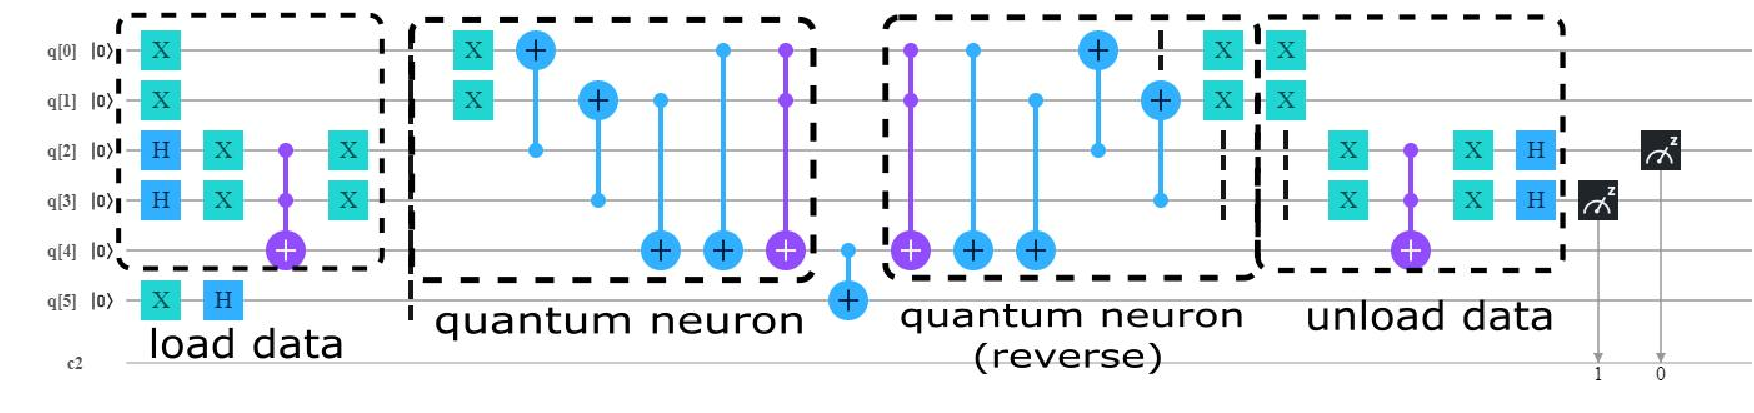
\includegraphics[width=9cm, scale=0.5]{images/circuit.pdf}
    \caption{This figure describes the evaluation procedure introduced in this section.
    The q[0] and q[1] are the weights, q[2] and q[3] are the inputs and the q[4] is the expected qubit
    and q[5] is the ancillary register of the Deutsch-Jozsa's algorithm.}\label{Fig:MV}
\end{figure}

\section{Quantum Binary Neural Networks Evaluation}\label{sec:quantum-binary-neural-networks-evaluation}

\subsection*{The Problem}\label{subsec:the-problem2}
 The problem proposed by~\cite{fawaz2019training} consists of given inputs \((x_1, x_2, x_3)\) the function
  \(sign(x_3*x_1, x_2)\) and \(sign(x_1 + x_2 + x_3)\) return 1 if the result is equal o greater than 0 and -1 otherwise.

 \subsection{Parameters Initialization}\label{subsec:initializaton}
   Given the initial states of the weights, inputs and the expected outcome defined as $|x\rangle$ and $|w\rangle$
 $|o\rangle$ respectively, we also have the ancillary qubit used in the Deutsch - Jozsa algorithm.\footnote[1]{
  An extra qubit must be added to load the data in the implementation process.}
 We define a quantum superposition of all possible inputs using the $H^ {\otimes n}$.
 Then the initial state is:

  \begin{equation}
          |\psi_0\rangle = |w\rangle|x_1, x_2, x_3\rangle|o\rangle
  \end{equation}

  \begin{equation}
          \rightarrow \sum_{x \in \{x_1, x_2, x_3\}^n}
          \frac{|w\rangle|x\rangle|o\rangle}{\sqrt{X}}\Bigg[\frac{0\rangle - |1\rangle}{\sqrt{2}}\Bigg]
  \end{equation}
  The inputs are represented in a binary form 1 and 0 for inputs 1 and -1 respectively.
  The inputs are three  $(x_1, x_2, x_3)$ and the expected result.
  The expected outcome can be loaded using the mct function available at qiskit.

\subsection{Quantum Neuron}\label{subsec:quantum-neuron}
  Now differently of~\cite{fawaz2019training} approach, we apply an specific set of weight to the inputs using the
  anti-C-not gate.
  At this step we must apply the activation function that is defined as the majority function.
 This function consists of given 1 if a binary inputs has more ones than zeros.
  Such process is done for every quantum neuron in the QBNN~\cite{fawaz2019training} proposal.

\subsection{Verification}\label{subsec:verification}
  Now we must apply a c-not gate where the expected outcome qubit is the control and Deutsch - Jozsa ancillary is the target.
 Then each state will flip the sign if the QBNN yield a correct answer and sign will stay the same otherwise.
 We can see it in the form of \((-1)^{f(x)}|x\rangle\), where the QBNN is our function.
 Further, we just need to undo the last operations and unload the data before the evaluation.
 After, we evaluate the outcome applying the $H^{\otimes n}$ in $(x_1, x_2, x_3)$ again and measuring the outcomes.

  % fazer nova imagem


\section{Experiments}\label{sec:experiments}

    We used the qiskit API~\cite{Qiskit} for the implementation of the QBNN algorithm.
    Further, we test all the possibility of 8 binary weights resulting in 256 simulations.
    The data was loaded using the mct function available at~\cite{Qiskit} with the addition with an ancillary qubit.\footnote{
   The mct or Multiple-Control Toffoli operation is a control operation like c-not generally used when you have more than
   two qubits as control and one target~\cite{Maslov_2016}
}
    The reverse operation explained in the last section is achieved applying the same operation in the reverse order.
    The figures 3 and 4 shows the relation of each weight (in the decimal representation)

    \begin{figure}[h!]
    \centering
    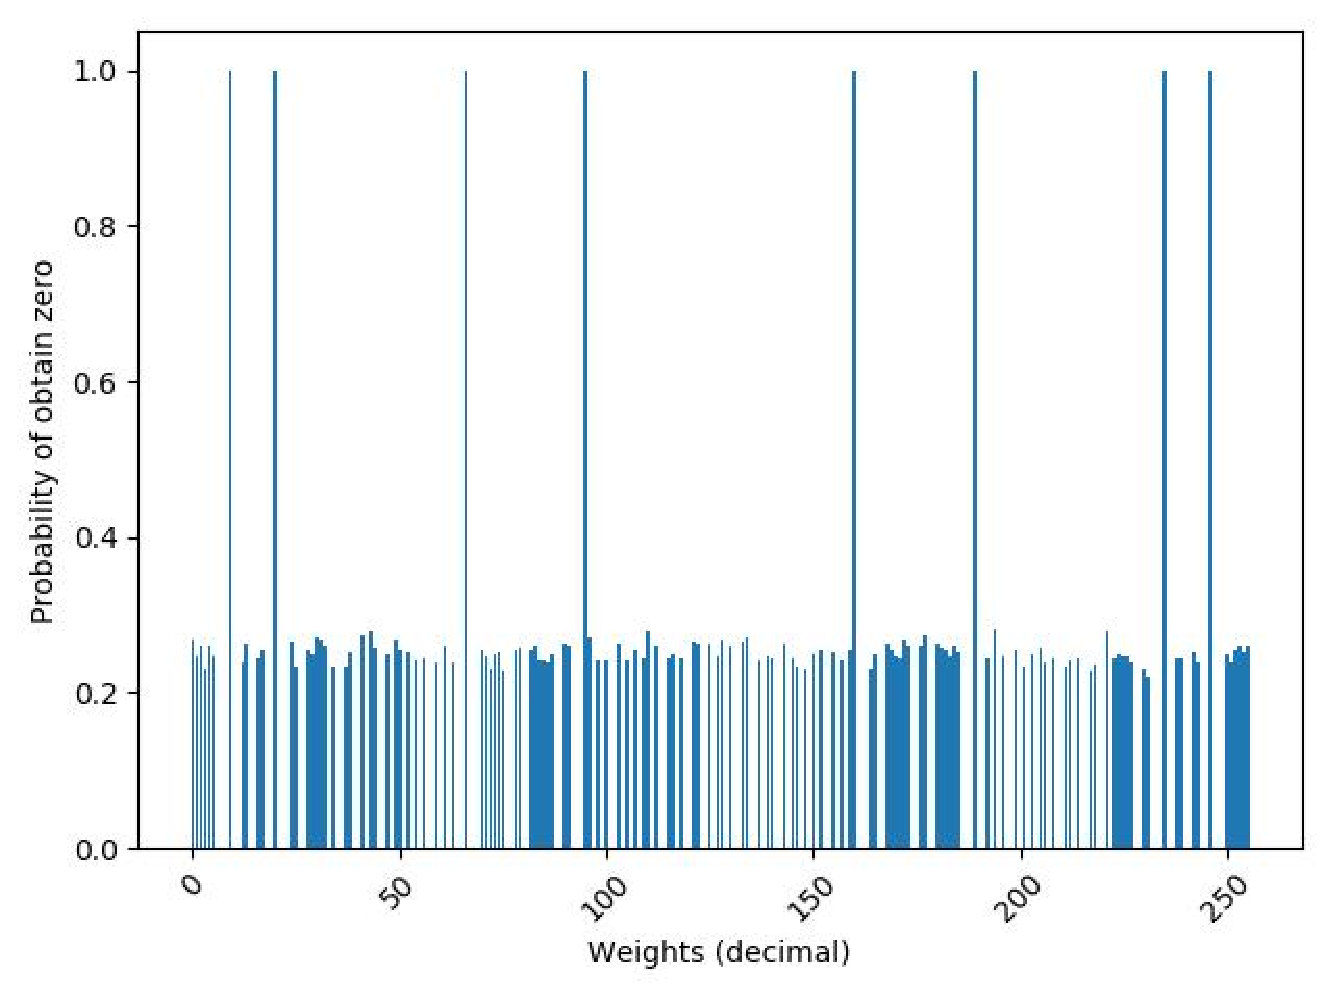
\includegraphics[width=9cm, scale=0.4]{images/problem_1.pdf}
    \caption{This represents the evaluation of all weights (in the decimal form) of the problem 1.
    As we can see a few of them produce a 100\% for the problem \(sign(x_3*x_1, x_2)\).}\label{Fig:problem_1}
    \end{figure}

    \begin{figure}[h!]
        \centering
        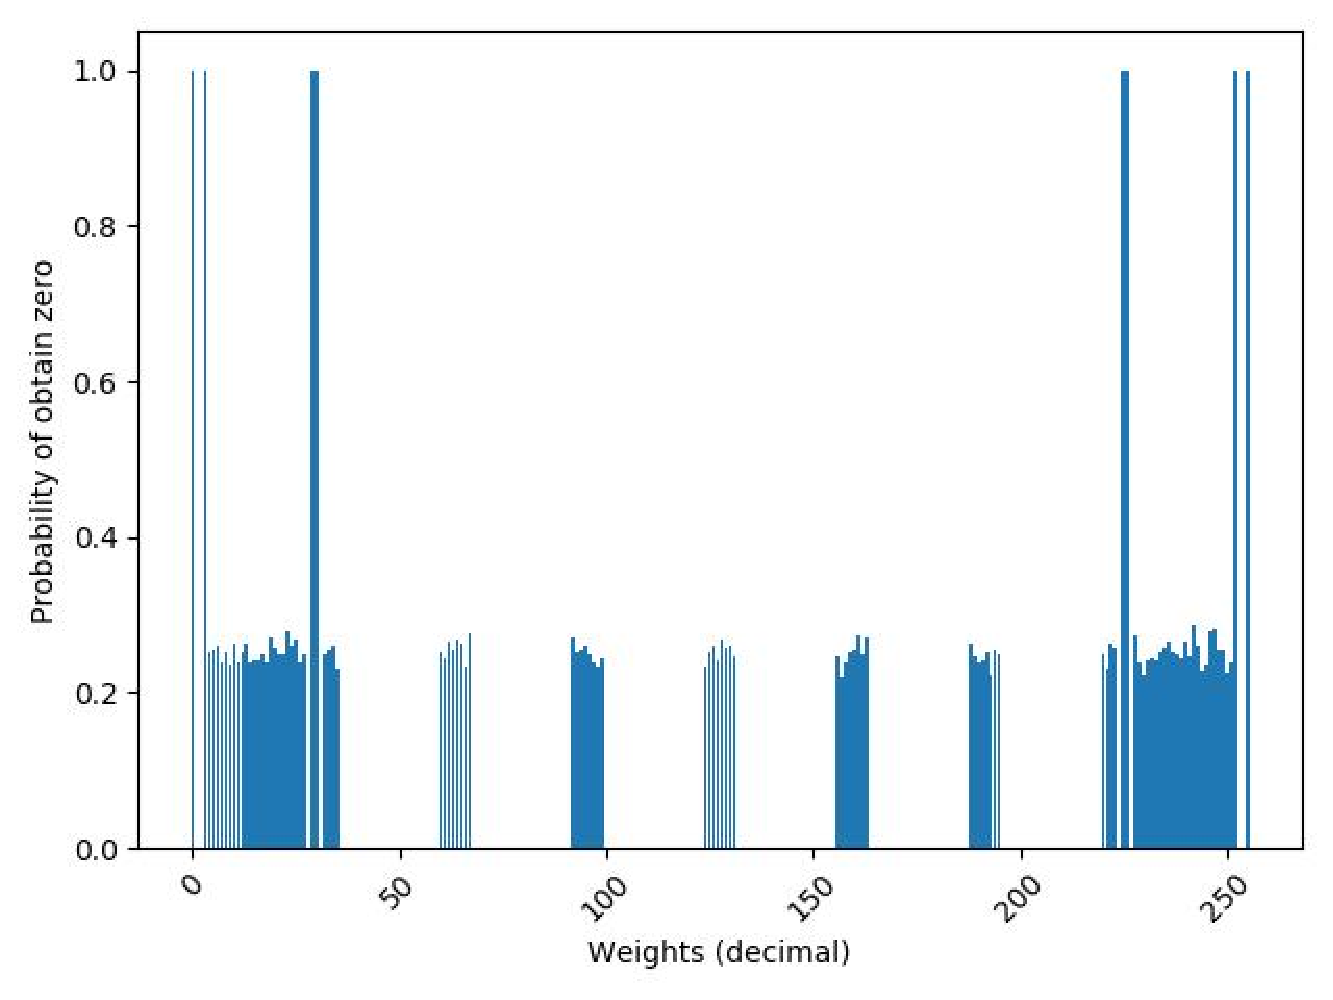
\includegraphics[width=9cm, scale=0.4]{images/problem_2.pdf}
        \caption{This represents the evaluation of all weights (in the decimal form) of the problem 1.
        As we can see a few of them produce a 100\% for the problem \(sign(x_1 + x_2 + x_3)\).}\label{Fig:problem_2}
    \end{figure}

\section{Discussion}\label{sec:discussion}
 The experiments shows that it was possible to identify specific weights that yields 100\% hits in the QBNN\@ rapidly.
It simply shows that it's possible to evaluate a given quantum neural binary network consuming less computational resources and
with less execution as proposed in the original paper~\cite{fawaz2019training}.
Considering that the today's quantum computer have a qubit constrain and a operation limitations;
it could be seen as an improvement in the efficiency of the QBNN allowing it to load a larger amount of data as it evaluate
a specific architecture.



\section{Conclusion}\label{sec:conclusion}

  In this work, we presented an possible method to extract probabilistic information about the accuracy of the
  Quantum Binary Neural Networks with a single call of the classifier.
  Based on the results, it is possible to verify that the Deutsch - Jozsa's algorithm would be a good option in terms
  of a rapid evaluation.
  As the first attempt to use Deutsch - Jozsa's algorithm to evaluate a QBNN some question must be addressed such as the
  noise influence in a real quantum device and the evaluation in the case of a QBNN that is neither constant nor balanced.
  Moreover, the Deutsch-Jozsa's algorithm could be used as method for quantum training the architecture selection because
  of its lower computational resource requirement and execution speed.

\bibliographystyle{unsrt}
\bibliography{references}

\end{document}
